%\FloatBarrier
\section{Topological Skeletons}
\label{sec:topology-skeletons}
Even though many algorithms can be expressed by parallel maps, some problems require more sophisticated skeletons. The Eden library leverages this problem and already comes with more predefined skeletons\footnote{Available on Hackage: \url{https://hackage.haskell.org/package/edenskel-2.1.0.0/docs/Control-Parallel-Eden-Topology.html}.}, among them a |pipe|, a |ring|, and a |torus| implementations \cite{Loogen2012}. These seem like reasonable candidates to be ported to our Arrow-based parallel Haskell. We aim to showcase that we can express more sophisticated skeletons with Parallel Arrows as well.

\subsection{Parallel pipe}\label{sec:pipe}

The parallel |pipe| skeleton is semantically equivalent to folding over a list |[arr a a]| of arrows with |>>>|, but does this in parallel, meaning that the arrows do not have to reside on the same thread/machine. We implement this skeleton using the |ArrowLoop| typeclass which gives us the |loop :: arr (a, b) (c, b) -> arr a c| combinator which allows us to express recursive fix-point computations in which output values are fed back as input. For example %this
\begin{code}
loop (arr (\(a, b) -> (b, a:b)))
\end{code}
which is the same as
\begin{code}
loop (arr snd &&& arr (uncurry (:)))
\end{code}
defines an arrow that takes its input |a| and converts it into an infinite stream |[a]| of it. Using this to our advantage gives us a first draft of a pipe implementation (Fig.~\ref{fig:pipeSimple}) by plugging in the parallel evaluation call |parEvalN conf fs| inside the second argument of |&&&| and then only picking the first element of the resulting list with |arr last|.

However, using this definition directly will make the master node a potential bottleneck in distributed environments as described in Section~\ref{futures}. Therefore, we introduce a more sophisticated version that internally uses Futures and obtain the final definition of |pipe| in Fig.~\ref{fig:pipe}.

\begin{figure}[t]
\begin{code}
pipeSimple :: (ArrowLoop arr, ArrowParallel arr a a conf) =>
	conf -> [arr a a] -> arr a a
pipeSimple conf fs =
	loop (arr snd &&&
		(arr (uncurry (:) >>> lazy) >>> parEvalN conf fs)) >>>
	arr last
\end{code}
\caption{A~first implementation of the |pipe| skeleton expressed with Parallel Arrows. Note that the use of |lazy| (Fig.~\ref{fig:edenlazyrightrotate}) is essential as without it programs using this definition would never halt. We need to enforce that the evaluation of the input |[a]| terminates before passing it into |parEvalN|.}
\label{fig:pipeSimple}

\begin{code}
pipe :: (ArrowLoop arr, ArrowParallel arr (fut a) (fut a) conf, Future fut a) =>
	conf -> [arr a a] -> arr a a
pipe conf fs = unliftFut (pipeSimple conf (map liftFut fs))
\end{code}
\caption{Final definition of the |pipe| skeleton with Futures.}
\label{fig:pipe}
\end{figure}


Sometimes, this |pipe| definition can be a bit inconvenient, especially if we want to pipe arrows of mixed types together, i.e. |arr a b| and |arr b c|. By wrapping these two arrows inside a common type we obtain |pipe2| (Fig.~\ref{fig:pipe2}).
\begin{figure}[tb]
\begin{code}
pipe2 :: (ArrowLoop arr, ArrowChoice arr, Future fut (([a], [b]), [c]),
         ArrowParallel arr (fut (([a], [b]), [c])) (fut (([a], [b]), [c])) conf) =>
	conf -> arr a b -> arr b c -> arr a c
pipe2 conf f g =
	(arr return &&& arr (const [])) &&& arr (const []) >>>
	pipe conf (replicate 2 (unify f g)) >>>
	arr snd >>> arr head where
			unify :: (ArrowChoice arr) => arr a b -> arr b c -> arr (([a], [b]), [c]) (([a], [b]), [c])
			unify f g =
				(mapArr f *** mapArr g) *** arr (\_ -> []) >>>
				arr (\((a, b), c) -> ((c, a), b))

(parcomp) :: (ArrowLoop arr, ArrowChoice arr, Future fut (([a], [b]), [c]),
	ArrowParallel arr (fut (([a], [b]), [c])) (fut (([a], [b]), [c])) ()) =>
	arr a b -> arr b c -> arr a c
(parcomp) = pipe2 ()
\end{code}
\caption{Definition of |pipe2| and a parallel |>>>|.}
\label{fig:pipe2}
\end{figure}
\mbcomment{parallel >>>!!!!!!}

Note that extensive use of |pipe2| over |pipe| with a hand-written combination data type will probably result in worse performance because of more communication overhead from the many calls to parEvalN. Nonetheless, we can define a version of parallel piping operator |parcomp|, which is semantically equivalent to |>>>| similarly to other parallel syntactic sugar from Appendix~\ref{syntacticSugar}.

Another version of |>>>| is:
\begin{code}
f parparcomp g = (f . put) >>> (get . g)
\end{code}
It does not launch both arrows |f| and |g| in parallel, but allows for more smooth data commuinication between them. Basically, it is a |Future|-lifted \emph{sequential} |>>>|, a way to compose parallel Arrows efficiently.

\subsection{Ring skeleton} \label{sec:ring}
\begin{figure}[tb]
	\includegraphics[scale=0.75]{images/ring}
	\caption{Schematic depiction of the ring skeleton.}
	\label{fig:ringImg}
\end{figure}
Eden comes with a ring skeleton\footnote{Available on Hackage: \url{https://hackage.haskell.org/package/edenskel-2.1.0.0/docs/Control-Parallel-Eden-Topology.html}} (Fig.~\ref{fig:ringImg}) implementation that allows the computation of a function |[i] -> [o]| with a ring of nodes that communicate in a ring topology with each other. Its input is a node function |i -> r -> (o, r)| in which |r| serves as the intermediary output that gets send to the neighbour of each node. This data is sent over direct communication channels, the so called \enquote{remote data}. We depict it in Appendix, Fig.~\ref{fig:ringEden}.
%\end{code}
%with toRD (to make use of remote data)
%\begin{code}
%\end{code}
%and rightRotate:
%\begin{code}


We can rewrite this functionality easily with the use of |loop| as the definition of the node function, |arr (i, r) (o, r)|, after being transformed into an arrow, already fits quite neatly into the |loop|'s |arr (a, b) (c, b) -> arr a c|. In each iteration we start by rotating the intermediary input from the nodes |[fut r]| with |second (rightRotate >>> lazy)| (Fig.~\ref{fig:edenlazyrightrotate}). Similarly to the |pipe| from Section~\ref{sec:pipe} (Fig.~\ref{fig:pipeSimple}), we have to feed the intermediary input into our |lazy| (Fig.~\ref{fig:edenlazyrightrotate}) arrow here, or the evaluation would fail to terminate. The reasoning is explained by \citet{Loogen2012} as a demand problem.

Next, we zip the resulting |([i], [fut r])| to |[(i, fut r)]| with |arr (uncurry zip)| so we can feed that into a our input arrow |arr (i, r) (o, r)|, which we transform into |arr (i, fut r) (o, fut r)| before lifting it to |arr [(i, fut r)] [(o, fut r)]| to get a list |[(o, fut r)]|. Finally we unzip this list into |([o], [fut r])|. Plugging this arrow |arr ([i], [fut r]) ([o], fut r)| into the definition of |loop| from earlier gives us |arr [i] [o]|, our ring arrow (Fig.~\ref{fig:ringFinal}).
This combinator can, for example, be used to calculate the shortest paths in a graph using Warshall's algorithm.
%Further details on this can be found in \cite{eden_cefp}.
\olcomment{let's do it?}


\begin{figure}[tb]
\begin{code}
ring :: (ArrowLoop arr, Future fut r, ArrowParallel arr (i, fut r) (o, fut r) conf) =>
    conf -> arr (i, r) (o, r) -> arr [i] [o]
ring conf f =
	loop (second (rightRotate >>> lazy) >>> arr (uncurry zip) >>>
        parMap conf (second get >>> f >>> second put) >>> arr unzip)
\end{code}
\caption{Final definition of the |ring| skeleton.}
\label{fig:ringFinal}
\end{figure}
 % $ %% formatting
% and lazy:
% \begin{code}
% lazy :: (Arrow arr) => arr [a] [a]
% lazy = arr (\ ~(x:xs) -> x : lazy xs
% \end{code}
%% we have shown this already.

\subsection{Torus skeleton}
\begin{figure}
	\includegraphics[scale=0.75]{images/torus}
	\caption{Schematic depiction of the |torus| skeleton.}
	\label{fig:ringTorusImg}
\end{figure}
If we take the concept of a ring from Section~\ref{sec:ring} one dimension further, we obtain a |torus| skeleton (Fig.~\ref{fig:ringTorusImg},~\ref{fig:torus}). Every node sends ands receives data from horizontal and vertical neighbours in each communication round.
With our Parallel Arrows we re-implement the |torus| combinator\footnote{Available on Hackage: \url{https://hackage.haskell.org/package/edenskel-2.1.0.0/docs/Control-Parallel-Eden-Topology.html}.} from Eden---yet again with the help of the |ArrowLoop| typeclass.

Similar to the |ring|, we once again start by rotating the input (Fig.~\ref{fig:edenlazyrightrotate}), but this time not only in one direction, but in two. This means that the intermediary input from the neighbour nodes has to be stored in a tuple |([[fut a]], [[fut b]])| in the second argument (loop only allows for two arguments) of our looped arrow |arr ([[c]], ([[fut a]], [[fut b]])) ([[d]], ([[fut a]], [[fut b]]))| and our rotation arrow becomes 
\begin{code}
second ((mapArr rightRotate >>> lazy) *** (arr rightRotate >>> lazy))
\end{code}
instead of the singular rotation in the ring as we rotate |[[fut a]]| horizontally and |[[fut b]]| vertically. Then, we once again zip the inputs for the input arrow with 
\begin{code}
arr (uncurry3 zipWith3 lazyzip3)
\end{code}
from |([[c]], ([[fut a]], [[fut b]]))| to |[[(c, fut a, fut b)]]|, which we then feed into our parallel execution.

This action is, however,  more complicated than in the ring case as we have one more dimension of inputs to be transformed. We first have to |shuffle| all the inputs to then pass it into |parMap conf (ptorus f)| which yields |[(d, fut a, fut b)]|. We can then unpack this shuffled list back to its original ordering by feeding it into the specific unshuffle arrow we created one step earlier with |arr length >>> arr unshuffle| with the use of |app :: arr (arr a b, a) c| from the |ArrowApply| typeclass. Finally, we unpack this matrix |[[[(d, fut a, fut b)]]| with |arr (map unzip3) >>> arr unzip3 >>> threetotwo| to get  |([[d]], ([[fut a]], [[fut b]]))|.

\begin{figure}[tb]
\begin{code}
torus :: (ArrowLoop arr, ArrowChoice arr, ArrowApply arr, Future fut a, Future fut b,
          ArrowParallel arr (c, fut a, fut b) (d, fut a, fut b) conf) =>
	conf -> arr (c, a, b) (d, a, b) -> arr [[c]] [[d]]
torus conf f =
	loop (second ((mapArr rightRotate >>> lazy) *** (arr rightRotate >>> lazy)) >>>
	arr (uncurry3 (zipWith3 lazyzip3)) >>>
	(arr length >>> arr unshuffle) &&& (shuffle >>> parMap conf (ptorus f)) >>> app >>>
	arr (map unzip3) >>> arr unzip3 >>> threetotwo)

ptorus :: (Arrow arr, Future fut a, Future fut b) =>
	arr (c, a, b) (d, a, b) -> arr (c, fut a, fut b) (d, fut a, fut b)
ptorus f = arr (\ ~(c, a, b) -> (c, get a, get b)) >>> f >>> arr (\ ~(d, a, b) -> (d, put a, put b))
\end{code} % $
\caption{Definition of the |torus| skeleton. The definitions of |lazyzip3|, |uncurry3| and |threetotwo| have been omitted and can be found in Fig.~\ref{fig:lazyzip3etc}}.
\label{fig:torus}
\end{figure}
As an example of using this skeleton \citep{Loogen2012} showed the matrix multiplication using the Gentleman algorithm (\citeyear{Gentleman1978}). Their instantiation of the skeleton |nodefunction| can be adapted as shown in Fig.~\ref{fig:torusMatMult}.
\begin{figure}[tb]
\begin{code}
nodefunction :: Int -> ((Matrix, Matrix), [Matrix], [Matrix]) -> ([Matrix], [Matrix], [Matrix])
nodefunction n ((bA, bB), rows, cols) = ([bSum], bA:nextAs , bB:nextBs)
		where bSum = foldl' matAdd (matMult bA bB) (zipWith matMult nextAs nextBs)
			     nextAs = take (n-1) rows
			     nextBs = take (n-1) cols
\end{code}
\caption{Adapted |nodefunction| for matrix multiplication with the |torus| from Fig.~\ref{fig:torus}.}
\label{fig:torusMatMult}
\end{figure}
If we compare the trace from a call using our arrow definition of the torus (Fig.~\ref{fig:torus_parrows_trace}) with the Eden version (Fig.~\ref{fig:torus_eden_trace}) we can see that the behaviour of the arrow version and execution times are comparable. We discuss further examples on larger clusters and in a more detail in the next section.
\begin{figure}[tb]
\olcomment{more nodes!!!}
	\centering
	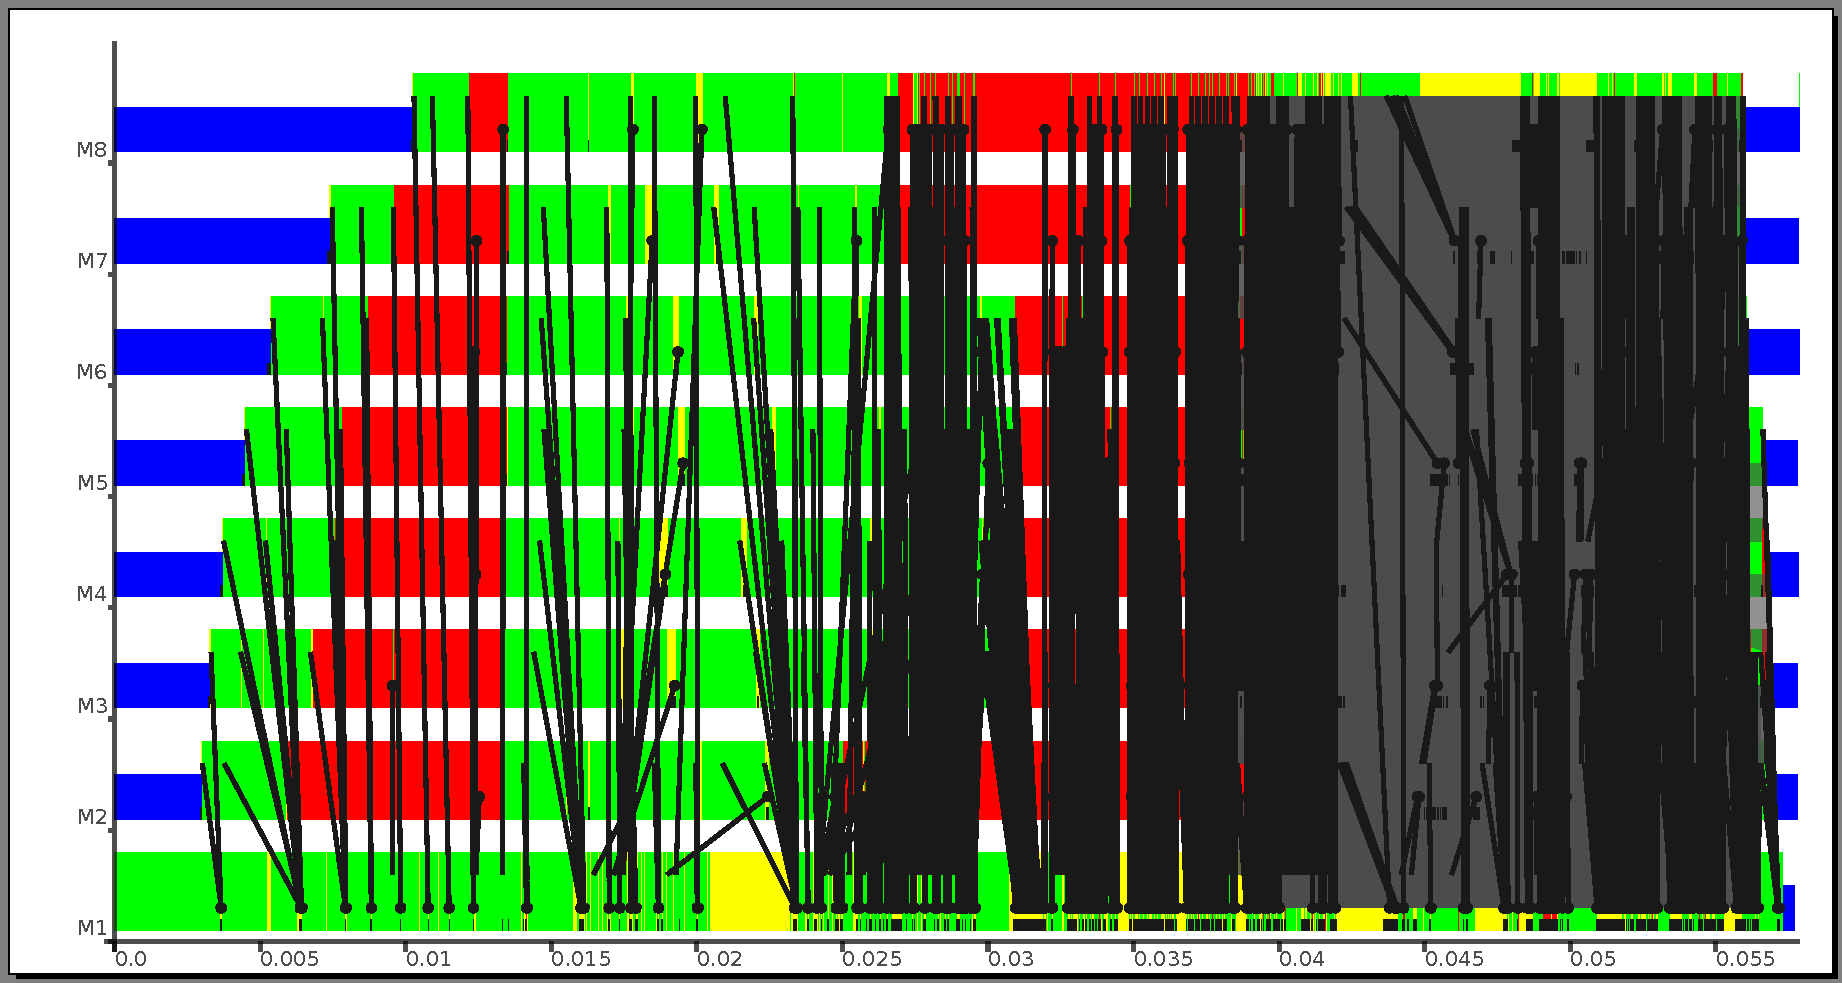
\includegraphics[width=0.9\textwidth]{images/torus_matrix_parrows_scale}
	\caption[Matrix Multiplication with a torus (Parrows)]{Matrix Multiplication with a torus (PArrows).}
	\label{fig:torus_parrows_trace}
\end{figure}

\begin{figure}[tb]
	\centering
	\includegraphics[width=0.9\textwidth]{images/torus_matrix_eden_scale}
	\caption[Matrix Multiplication with a torus (Eden)]{Matrix Multiplication with a torus (Eden).}
	\label{fig:torus_eden_trace}
\end{figure}

%\FloatBarrier

%%% Local Variables:
%%% mode: latex
%%% TeX-master: "main"
%%% End:
